\subsection{Versuchsaufbau}
\label{sec:Versuchsaufbau}
\begin{wrapfigure}{R}{5cm}
  \centering
  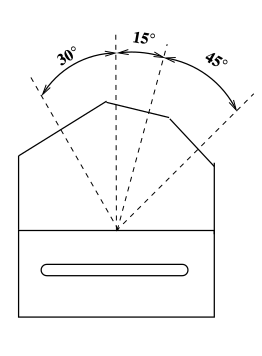
\includegraphics[width=0.25\textwidth]{Bilder/prisma.png}
  \caption{Schematische Darstellung des verwendeten Dopplerprisma. \cite{Anleitung}}
  \label{fig:dopplerprisma}
\end{wrapfigure}
Der Versuchsaufbau besteht zum Einen aus einer Strömungsröhre mit drei verschiedenen
Innendurchmessern ($\SI{7}{\milli\meter}$, $\SI{10}{\milli\meter}$ und $\SI{16}{\milli\meter}$).
Die Strömungsröhre ist mit einem Gemisch aus Wasser, Glycerin und Glaskugeln gefüllt.
Den drei Teilrohren ist jeweils ein Doppler-Prisma (vgl. Abbildung
\ref{fig:dopplerprisma}) zugeordnet, dessen drei Flächen den festen Winkeln $\SI{15}{\degree}$,
$\SI{30}{\degree}$ und $\SI{60}{\degree}$ entsprechen. Hiermit können drei feste Dopplerwinkel $\alpha$ bezüglich der Dopplerflüssigkeit realisiert werden, welche sich nach Formel \eqref{eqn:dopplerwinkel} berechnen.
Des Weiteren wird ein Ultraschall Doppler-Generator, eine Ultraschallsonde (Frequenz
$\SI{2}{\mega\hertz}$) und ein Rechner mit dem Programm FlowView verwendet, um die Messungen
aufzunehmen. Außerdem wird eine Zentrifugalpumpe gebraucht, mit der die
Strömungsgeschwindigkeit
varriert wird.
